\documentclass[a4paper,11pt]{article}
\usepackage{commonpackages}

\usepackage{xcolor}
\definecolor{mybackcolor}{rgb}{0.98,0.98,0.98}

\lstset{language=HTML, basicstyle={\small\ttfamily}, keywordstyle=\color{blue}, identifierstyle=\color{darkgray}, stringstyle=\color{brown}, backgroundcolor=\color{mybackcolor}, numbers=left}

\begin{document}
\title{HTML}
\date{}
\maketitle

\section{Introduction}
\subsection{Web et Internet}
Internet ne doit pas être confondu avec le World Wide Web. Ces deux mots ne sont pas des synonymes.\\
\textbf{Internet} est le réseau physique (filaire ou par ondes) qui relie les ordinateurs entre eux et qui permet aux ordinateurs de communiquer entre eux.
Le \textbf{World Wide Web} qui signifie la toile d'araignée mondiale (abrégé Web) est un ensemble de pages, de documents et de ressources publiques, tous reliés les uns aux autres par des liens hypertextes. Le Web fonctionne sur le réseau internet. Le Web a été créé au CERN à Genève en 1989.\\
Les navigateurs (Browser en anglais) comme Firefox, Chrome, Safari, \dots sont des logiciels conçus pour consulter et afficher les données du Web sur notre ordinateur.

\subsection{Système Client-Serveur}
Le Web est basé sur un modèle client-serveur. Le navigateur est un client qui demande un site Web à un serveur. Le serveur est un ordinateur qui fournit des services sur un réseau. Dans notre cas, le serveur stocke les différents sites Web et envoie le fichier HTML demandé au client, c'est un serveur Web.
\begin{enumerate}[label=\arabic*)]
\item L'utilisateur entre l'adresse d'un site Web, appelée URL (Uniform Resource Locator).
\item Cette requête va être transmise via internet au serveur Web.
\item Lorsque le serveur Web reçoit la requête, il transmet le fichier HTML correspondant à la demande au client via internet.
\item Le navigateur va lire et interpréter le fichier HTML pour pouvoir l'afficher sur l'écran de l'utilisateur.
\end{enumerate}
\video[100]{dYgNvn98Nag}

\section{Fichiers d'une page Web}
Une page Web est typiquement composée de 3 types de fichiers:
\begin{enumerate}[label=\arabic*)]
\item HTML
\begin{itemize}
  \item Contenu (texte, images, liens, etc.)
  \item Structure (titre, sous-titres, paragraphes, etc.)
\end{itemize}
\item CSS
\begin{itemize}
  \item Style (couleurs, police d'écriture, alignement, taille des éléments, etc.)
\end{itemize}
\item JavaScript
\begin{itemize}
  \item Permet de rendre la page Web dynamique (la page change en fonction des actions effectuées)
\end{itemize}
\end{enumerate}
\video[100]{-7pJ45oXuvE}

\section{Définition du format HTML}
Le format \textbf{HTML} (HyperText Markup Language) est un format qui permet de décrire le contenu et la structure d'une page Web. HTML n'est pas un langage de programmation, il ne contient ni fonction, ni boucle, ni instruction conditionnelle, mais c'est un ensemble de balises qui permettent de mettre un document en page, afin que le navigateur puisse l'afficher correctement.

\subsection{Balises}
Les balises ont la forme suivante:
\begin{verbatim}{html}
<h1>Bienvenue sur notre site Web</h1>
\end{verbatim}
<h1> est une balise ouvrante et </h2> est une balise fermante. À chaque balise ouvrante correspond une balise fermante à l'exception des balises qui n'ont pas de contenu.

\subsection{Balise <!DOCTYPE html>}
Tous documents qui décrivent une page Web doivent débuter par:  <!DOCTYPE html>
Ce n'est pas une balise HTML, mais une information qui permet au navigateur de savoir le type de document.

\subsection{Balise <html> \dots <html>}
Tout le code HTML doit être inséré dans une balise nommée html: <html> … </html>
La balise html contient en général deux autres balises:
\begin{itemize}
\item <head> … </head>\\
entête du document, elle contient différentes informations concernant le document (titre de la page, type d'encodage, lien vers le fichier CSS, etc.).
Ces informations ne seront pas affichées à l'écran à l'exception du titre affiché sur l'onglet de la page.
\item <body> … </body>\\
contient le contenu (corps) de la page. Tout ce qui sera dans cette partie sera affiché.
\end{itemize}
\begin{multicols}{2}
\begin{verbatim}{html}
<!DOCTYPE html>
<html>
  <head>
   ...
  </head>
  <body>
   ...
  </body>
</html>
\end{verbatim}
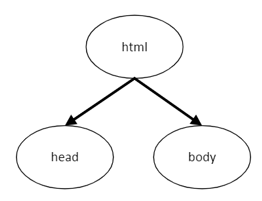
\includegraphics[width=0.6\textwidth]{images/balise-html.png} \\
\end{multicols}

\newpage

\subsection{Balise <body> \dots <body>}
Dans la balise body, nous allons structurer le contenu de la page. Nous allons voir les balises les plus simples qui permettent de définir des titres, sous-titres et paragraphes:
\begin{itemize}
\item <h1> \dots </h1>  permet de définir un titre principale
\item <h2> \dots </h2>  permet de définir un sous-titre
\item <h3> \dots </h3>  permet de définir un sous-sous-titre
\item <h\dots> \dots </h\dots>  permet de définir  sous-\dots-sous-titre
\item  <p> \dots </p>  permet de définir un paragraphe
\end{itemize}
\begin{multicols}{2}
\begin{verbatim}{html}
<!DOCTYPE html>
<html>
  <head> ... </head>
  <body>
    <h1>Titre principal</h1>
    <p>Le paragraphe</p>
  </body>
</html>
\end{verbatim}
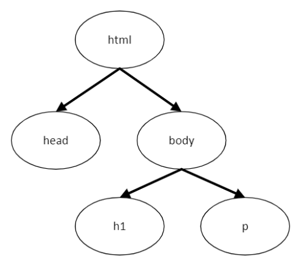
\includegraphics[width=0.5\textwidth]{images/balise-body.png} \\
\end{multicols}

\subsection{Balise <head> \dots <head>}
La balise head contient différentes informations sur le document, notamment le titre de la page et le type d'encodage.

\subsubsection{Balise <title> \dots <title>}
La balise title permet de définir le titre de la page qui s'affichera sur l'onglet du navigateur web.
\begin{verbatim}{html}
<title>Ma page</title>
\end{verbatim}

\includegraphics[width=1.0\textwidth]{images/barre-titre.png}

\subsubsection{Balise <meta>}
La balise meta permet d'indiquer le type d'encodage (ASCII, Unicode, UTF-8). Nous souhaitons que les accents s'écrire correctement sur notre page, nous allons donc utiliser de l'utf-8 que nous allons indiquer dans l'attribut charset:
\begin{verbatim}{html}
<meta charset="utf-8">
\end{verbatim}
Comme cette balise ne contient pas de contenu, c'est une balise unique (pas de balise ouvrante et fermante).

\section{Exercices}
\subsection{Exercice 1}
But: Comprendre la structure principale d'un document HTML.
Faire l'ex 1 sur Moodle: \url{https://moodle.fritic.ch/mod/hvp/view.php?id=112347}

\subsection{Exercice 2}
But: Ouvrir un document HTML sur replit.com.
\begin{multicols}{2}
\begin{enumerate}[label=\arabic*)]
\item Sur Moodle, télécharger le document \textbf{index.html}.
\item Sauvegarder ce document sur OneDrive dans le dossier informatique.
\item Se connecter sur replit.com.
\item Cliquer sur \textbf{+ Create Repl}.
\item Choisir \textbf{HTML, CSS, JS}.
\item Nommer le Repl \textbf{Exemple}.
\end{enumerate}
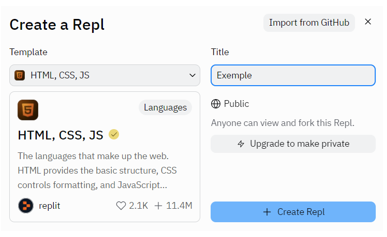
\includegraphics[width=1\textwidth]{images/replit.png} \\
\end{multicols}
\begin{enumerate}[label=\arabic*)]\addtocounter{enumi}{6}
\item Cliquer à nouveau sur \textbf{+ Create Repl}.
\item Il faut remplacer le fichier index.html par celui que vous avez téléchargé:
\begin{enumerate}
  \item Effacer le fichier « index.html » déjà présent.
  \item Télécharger votre fichier en cliquant sur les 3 points verticaux et en séléctionnant \textbf{Upload file}. Choisir le fichier textbf{index.html} que vous avez sauvergarder sur votre OneDrive.
\end{enumerate}
\item Appuyer sur le bouton \textbf{Run}.
\end{enumerate}

\subsection{Exercice 3}
Vous voyez maintenant le code HTML et ce que la page affiche.
\begin{enumerate}[label=\arabic*)]
\item Qu'est-ce que vous comprenez de cette page?
\item Vous allez maintenant modifier cette page (pour valider une modification, appuyer sur \textbf{Run}:
\begin{enumerate}
  \item Modifier le titre et le premier paragraphe pour remplacer Collège du Sud par Collège Sainte-Croix.
  \item Modifier la partie présentation pour avoir les informations qui correspondent au Collège Sainte-Croix. Changer aussi le lien vers le site de l'école. (cf. 3.6)
  \item Compléter la liste de vos cours avec: Économie et droit, Biologie, \dots
  \item Changer la liste de vos cours par une liste numérotée. (cf. 3.7.1)
  \item Ajouter un sous-titre \textbf{Ma classe} et un paragraphe avec quelques informations.
  \item Ajouter une image du Collège Sainte-Croix:
\begin{enumerate}[label=\roman*.]
    \item Télécharger l'image que vous avez choisie.
    \item Importer l'image sur replit.com dans un répertoire nommé \textbf{images}.
    \item Noter le code HTML nécessaire. (cf. 3.8)
  \item Ne pas oublier d'indiquer la source.
\end{enumerate}
\end{enumerate}
\end{enumerate}

\section{Solution}

\lstset{identifierstyle=\color{black}, commentstyle=\color{gray}}

\subsection{Exercice 3}
1) Fichier index.htlm
\begin{verbatim}{html}
<!DOCTYPE html> <!-- indique le genre de document au browser -->
<html>
  <head> <!-- métadonnées de la page et le titre de l'onglet -->
    <meta charset="utf-8">
    <title>Nom de la page</title>
  </head>
  <body> <!-- partie qui sera affichée -->
    <h1>Le collège du Sud</h1> <!-- titre principal -->
    <!-- 1er paragraphe -->
    <p>Voici ma première page Web sur le collège du Sud!</p>
    <h2>Présentation</h2> <!-- Sous-titre -->
    <!-- 2e paragraphe -->
    <p>
    Le Collège du Sud est un établissement fribourgeois du
    secondaire du 2e degré. Il offre actuellement 3 filières
    d’études : un gymnase, une école de commerce et une école
    de culture générale. Il reçoit des étudiant-e-s de 16 à 20 ans,
    qui proviennent essentiellement des districts de la Gruyère
    et de la Veveyse, mais aussi de la Glâne.</p>
    <!-- Ajout d'une image -->
    <p id="source">Source:
    <a href="https://collegedusud.ch/presentation/" target="_blank">
    Site internet du collège du Sud</a>
    <p/>
    <h2>Mes cours</h2> <!-- Sous-titre -->
    <ul> <!-- liste non numérotée -->
      <li>Français</li>
      <li>Allemand</li>
      <li>Anglais</li>
      <li>Maths</li>
    </ul>
  </body>
</html>
\end{verbatim}
2) Fichier index.html modifié
\begin{verbatim}{html}
<!DOCTYPE html>
<html>
  <head>
    <meta charset="utf-8">
    <title>Nom de la page</title>
  </head>
  <body>
    <h1>Le collège Sainte-Croix</h1>
    <p>Voici ma première page Web sur le collège Sainte-Croix!</p>
    <h2>Présentation</h2>
    <p>
    Le Collège Sainte-Croix est un établissement fribourgeois
    du secondaire du 2e degré. C'est un gymnase en ville de Fribourg
    qui permet de faire une maturité en français, en allemand ou un
    mixte des deux langues. Il reçoit des étudiant-e-s de 16 à 20 ans.
    </p>
    <p id="source">Source:
    <a href="https://new.cscfr.ch/index.php/fr/" target="_blank">
    Site internet du collège Sainte-Croix</a><p/>
    <h2>Mes cours</h2>
    <ol>
      <li>Français</li>
      <li>Allemand</li>
      <li>Anglais</li>
      <li>Maths</li>
      <li>Économie et droit</li>
      <li>Biologie</li>
      <li>...</li>
    </ol>
    <h2>Ma classe</h2>
    <p>
    Je fais partie de la classe 1F... qui est une classe qui ...
    <p/>
    <img src="images/STX.jpg" width="600" height="400"><br/>
    Source:
    <a href="https://new.cscfr.ch/index.php/fr/notre-college/">
    https://new.cscfr.ch/index.php/fr/notre-college/</a>
  </body>
</html>
\end{verbatim}

\subsection{Hyperlien <a href="\dots">}
La balise a permet de créer un  hyperlien, c'est-à-dire un texte sur lequel il faut cliquer pour accéder à une autre page. Il faut indiquer le lien dans l'attribut href:
<a href="lien">Texte</a>
\begin{verbatim}{html}
<p>
  Pour accéder au site du collège,
  cliquez <a href="https://www.cscfr.ch/index.php/fr/">ici</a>
</p>
\end{verbatim}
Pour ouvrir la nouvelle page dans un nouvel onglet, il faut ajouter l'attribut target avec la valeur \_blank:
\begin{verbatim}{html}
<a href="lien" target="_blank">Texte</a>
\end{verbatim}
Tuto: \href{https://developer.mozilla.org/fr/docs/Web/HTML/Element/a}{MDN - hyperliens}

\subsection{Listes}
Il existe deux types de listes:
\subsubsection{Listes numérotées (ordered) <ol>}
\begin{verbatim}{html}
<ol>
  <li>Mettre 1L d'eau dans un casserole</li>
  <li>Porter à ébullition</li>
  <li>...<\li>
</ol>
\end{verbatim}

\subsubsection{Listes à puces (unordered) <ul>}
\begin{verbatim}{html}
<ul>
  <li>Tomates</li>
  <li>Courgettes</li>
  <li>...<\li>
</ul>
\end{verbatim}
Tuto: \href{https://developer.mozilla.org/fr/docs/Web/HTML/Element/li}{MDN - listes}

\subsection{Image <img \dots>}
La balise img permet d'insérer une image sur une page Web. Dans l'attribut src, il faut indiquer le lien vers l'image, soit une URL, soit le chemin local.
\begin{verbatim}{html}
<img src = "mon_image.png"> (dans le même répertoire)
<img src= "images/mon_image.png"> (dans un sous-répertoire)
\end{verbatim}
Cette balise peut contenir aussi les attributs height ou width qui permettent de déterminer la hauteur et/ou la largeur de l'image en pixels.
\begin{verbatim}{html}
<img src= "images/mon_image.png" width="300" height="200">
\end{verbatim}
Tuto: \href{https://developer.mozilla.org/fr/docs/Learn/HTML/Multimedia_and_embedding/Images_in_HTML}{MDN - images}

\subsection{Saut de ligne <br/>}
La balise br permet de faire un saut de ligne (break). Comme cette balise ne contient pas de contenu, c'est une balise unique (pas de balise ouvrante et fermante).

\subsection{Tables ou tableaux}
La balise <table> permet de représenter des tableaux de données (tableaux en deux dimensions). Les tableaux peuvent aussi être utilisés pour la mise en page, par exemple mettre du texte à côté d'une image ou mettre plusieurs images l'une à côté de l'autre.
\begin{verbatim}{html}
<table>
  <tr>
    <td>Ingrédients</td>
    <td>Quantité</td>
  </tr>
  <tr>
    <td>Pommes de terre</td>
    <td>1 kg</td>
  </tr>
  <tr>
    <td>lait</td>
    <td>0.5l</td>
  </tr>
</table>
\end{verbatim}
Tuto: \href{https://developer.mozilla.org/fr/docs/Web/HTML/Element/table}{MDN - tables}\par

Suite du cours: \href{http://127.0.0.1:8000/doc/Informatique/HTML}{CSS}
\end{document}
